
\section{Implimentation}

\subsection{Training Model}

\begin{frame}  
    \frametitle{Training Model}
	\begin{itemize}
		\item Use keras
		\item Three dense layers each has 512 neurals
		\item 98 percent accuracy
	\end{itemize}
\end{frame}

\begin{frame}
	\frametitle{Training Model}
	\begin{figure}
		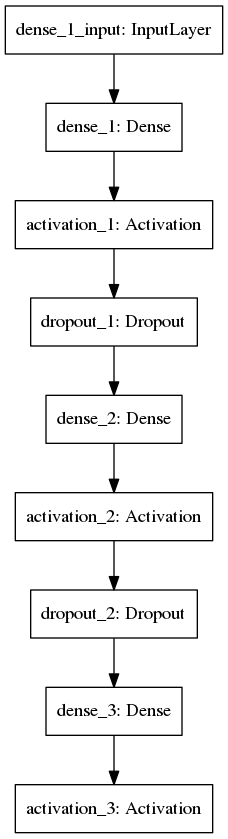
\includegraphics[scale=0.2]{figure/model_structure.png}
	\end{figure}
\end{frame}
\subsection{Server Synchronization}
\begin{frame}  
    \frametitle{Server Synchronization}
	\begin{itemize}
  		\item Synchronize client iterations	
		\item Python client, C server
		\item Two states machine		
		\begin{itemize}
  			\item Push state
			\item Pull state	
		\end{itemize}
	\end{itemize}
\end{frame}




